\documentclass[a4paper,parskip,11pt, DIV12]{scrreprt}

\usepackage[english]{babel} % Für Deutsch [english] zu [ngerman] ändern. 
\usepackage[utf8]{inputenc}
\usepackage[T1]{fontenc}
\usepackage{blindtext}
\usepackage{graphicx}
\usepackage{subfigure}
\renewcommand{\familydefault}{\sfdefault}
\usepackage{helvet}
\usepackage{fancyhdr}
\usepackage{amsmath}
\usepackage{mdwlist} %Benötigt für Abstände in Aufzählungen zu löschen
\usepackage{here}
\usepackage{calc}
\usepackage{hhline}
\usepackage{marginnote}
\usepackage{chngcntr}
\usepackage{tabularx}
\usepackage{titlesec} % Textüberschriften anpassen

% \titleformat{Überschriftenklasse}[Absatzformatierung]{Textformatierung} {Nummerierung}{Abstand zwischen Nummerierung und Überschriftentext}{Code vor der Überschrift}[Code nach der Überschrift]

% \titlespacing{Überschriftenklasse}{Linker Einzug}{Platz oberhalb}{Platz unterhalb}[rechter Einzug]

\titleformat{\chapter}{\LARGE\bfseries}{\thechapter\quad}{0pt}{}
\titleformat{\section}{\Large\bfseries}{\thesection\quad}{0pt}{}
\titleformat{\subsection}{\large\bfseries}{\thesubsection\quad}{0pt}{}
\titleformat{\subsubsection}{\normalsize\bfseries}{\thesubsubsection\quad}{0pt}{}

\titlespacing{\chapter}{0pt}{-2em}{6pt}
\titlespacing{\section}{0pt}{6pt}{-0.2em}
\titlespacing{\subsection}{0pt}{5pt}{-0.4em}
\titlespacing{\subsubsection}{0pt}{-0.3em}{-1em}

%\usepackage[singlespacing]{setspace}
%\usepackage[onehalfspacing]{setspace}

\usepackage[
%includemp,				%marginalien in Textkörper einbeziehen
%includeall,
%showframe,				%zeigt rahmen zum debuggen		
marginparwidth=25mm, 	%breite der marginalien
marginparsep=5mm,		%abstand marginalien - text
reversemarginpar,		%marginalien links statt rechts
%left=50mm,				%abstand von Seitenraendern
%			top=25mm,				%
%			bottom=50mm,
]{geometry}		

%Bibliographie- Einstellungen
\usepackage[babel,german=quotes]{csquotes}
\usepackage[
backend=bibtex8, 
natbib=true,
style=numeric,
sorting=none
]{biblatex}
\bibliography{Quelle}
%Fertig Bibliographie- Einstellungen

\usepackage{hyperref}

\newenvironment{conditions}
{\par\vspace{\abovedisplayskip}\noindent\begin{tabular}{>{$}l<{$} @{${}={}$} l}}
	{\end{tabular}\par\vspace{\belowdisplayskip}}
	
\begin{document}
	
	\begin{titlepage}
		\begin{figure}[H]
			\hfill
			\subfigure{
\includegraphics[scale=0.04]{uzh}}
		\end{figure}
		\vspace{1 cm}
		\textbf{\begin{huge}KT I Lab Course
		\end{huge}}\\
		\noindent\rule{\textwidth}{1.1 pt} \\
		
		\begin{Large}\textbf{Angular Correlation}
		\end{Large}\\ 
		\normalsize 
		\par
		\begingroup
		\leftskip 0 cm
		\rightskip\leftskip
		\textbf{Assistant:}\\ Alexander Kish \\ \\
		\textbf{Students:}\\ Fabian Stäger, Manuel Sommerhalder \\ \\
		\textbf{Date of experiment:}\\ 24.01.2018 \\ \\
		\par
		\endgroup
		\clearpage
		
		
		
	\end{titlepage}
	
%Start Layout
	\pagestyle{fancy}
	\fancyhead{} 
	\fancyhead[R]{\small \leftmark}
	\fancyhead[C]{\textbf{Angular Correlation} } 
	\fancyhead[L]{
\includegraphics[height=2\baselineskip]{uzh}}
	
	\fancyfoot{}
	\fancyfoot[R]{\small \thepage}
	\fancyfoot[L]{}
	\fancyfoot[C]{}
	\renewcommand{\footrulewidth}{0.4pt} 
	
	\addtolength{\headheight}{2\baselineskip}
	\addtolength{\headheight}{0.6pt}
	
	
	\renewcommand{\headrulewidth}{0.6pt}
	\renewcommand{\footrulewidth}{0.4pt}
	\fancypagestyle{plain}{				% plain redefinieren, damit wirklich alle seiten im gleichen stil sind (ausser titlepage)
		\pagestyle{fancy}}
	
	\renewcommand{\chaptermark}[1]{ \markboth{#1}{} } %Das aktuelle Kapitel soll nicht Gross geschriben und Nummeriertwerden
	
	\counterwithout{figure}{chapter}
	\counterwithout{table}{chapter}
	%Ende Layout
	
	\tableofcontents
	
\chapter{Introduction}

		The goal of this experiment is to measure the angular correlation function of $\gamma$-rays in a $^{60}$Co decay and compare it to theoretical predictions.

\section{The $^{60}$Co Decay}

		$^{60}$Co is a synthetic isotope of cobalt with a half-life of 5.1 years. Through $\beta ^-$ decay it disintegrates into an excited $^{60}$Ni atom with an energy of 2505 keV and $l$ = 4 with positive parity. This nickel isotope thus emits two successive gamma rays with energies of 1172 keV and 1332 keV in order to reach its stable state of 0$^{+}$. Since the intermediate state (2$^+$) has a lifetime of around 1 ps, the two $\gamma$-rays can due to the finite experimental time resolution be treated as coincident. A schematic diagram of the $^{60}$Co decay is provided in figure \ref{fig:CoDecay}.	
\begin{figure}[H]
\centering
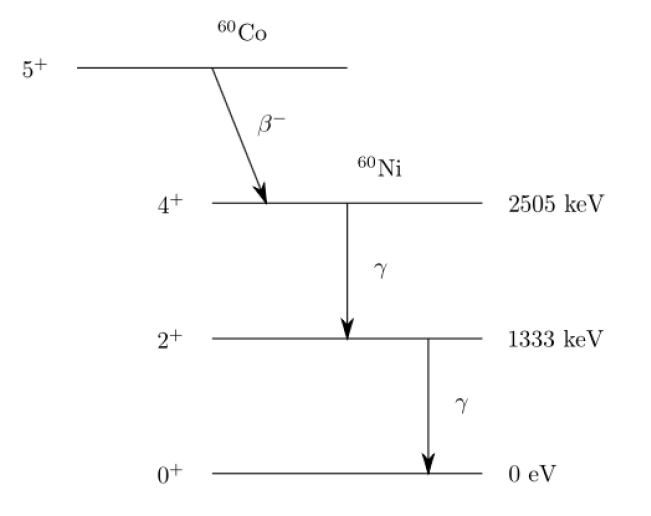
\includegraphics[scale=0.65]{60CoDecay.png}
\caption[60CoDecay]{Schematic illustration of the $^{60}$Co Decay. [\ref{source:manual}]}
\label{fig:CoDecay}
\end{figure}
		
\section{Angular Correlation}

		The two successive $\gamma$-rays are predicted to be emitted anisotropically relative to each other according to the general angular correlation function [\ref{source:manual}]:
		\begin{equation}
		W(\theta) = 1 + \sum^l_1 a_i \cos ^{2i} \theta
		\end{equation}	
		This function describes the probability for the latter gamma ray to be emitted at an angle $\theta$ from the first one. 2$l$ is the order of the lowest multipole in the cascade. In case of the $^{60}$Co decay, both gamma rays are emitted during a transision of $\Delta l$ = 2 and positive parity, so the dominant contribution is the electric quadrupole and the correlation function reduces to:	
		\begin{equation}
		W(\theta) = 1 + a_1 \cos ^{2} \theta +  a_2 \cos ^{4} \theta
		\end{equation}		
		The coefficients $a_1$ and $a_2$ have been theoretically predicted by Dr. Hamilton for all combinations of angular momenta involved by consideration of state transitions using the Clebsch-Gordan-coefficients. These are summarized in figure \ref{fig:coefficients}		
		\begin{figure}[H]
\centering
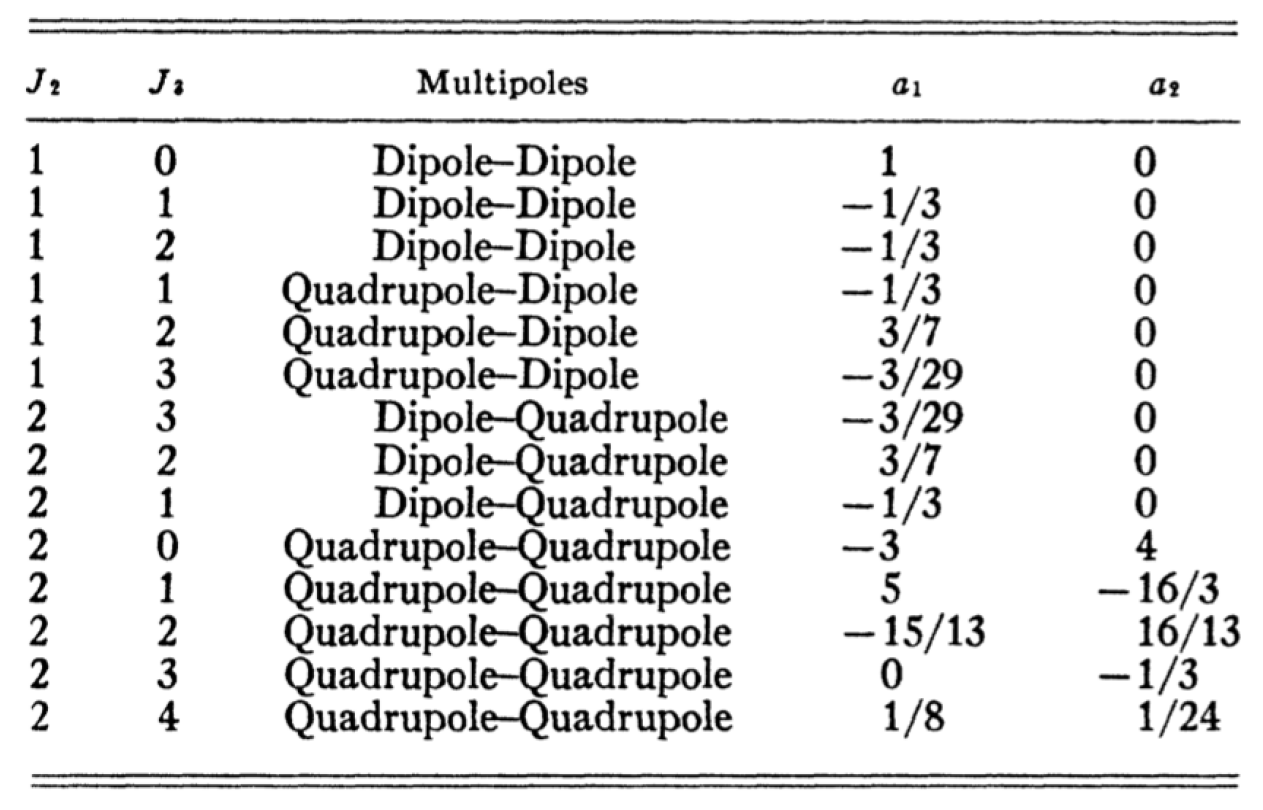
\includegraphics[scale=0.4]{Coefficients.png}
\caption[Coefficients]{Coefficients $a_1$ and $a_2$ for different combinations of $J_1$ and $J_2$ for an atom deexciting into the ground state $J_1$ = 0 [\ref{source:manual}]}
\label{fig:coefficients}
		\end{figure}		
		Since the angular monenta of $J_3$ = 4, $J_2$ = 2, $J_1$ = 0 are assumed for the $^{60}$Co decay, the expected correlation function has the following explicit form:		
		\begin{equation} \label{eq:AngularCorrelation}
		W(\theta) = 1 + \frac{1}{8} \cos ^{2} \theta +  \frac{1}{24} \cos ^{4} \theta
		\end{equation} 
		
\section{Experimental Concept}

		The experimental setup, more throroughly described in section \ref{sec:setup}, consists of two scintillation counters that detect the coincident $\gamma$-rays from different and adjustable relative angles. The rate of detected events is then plotted and compared to the theoretical description from formula \ref{eq:AngularCorrelation}.
		
\chapter{Measurement Principle}	

\section{Experimental Set-Up}

\section{Electronic Modules}

\chapter{Energy Spectrum}

\chapter{Calibration}

\end{document}